\documentclass[spanish]{report}

% -------------------------
% PAQUETES GENERALES
% -------------------------
\usepackage[utf8]{inputenc}       % Codificación UTF-8
\usepackage[spanish]{babel}       % Configuración del idioma en español
\usepackage{graphicx, tikz, amsmath, amssymb, xcolor, fancyhdr, svg, geometry, hyperref, csquotes}
\usepackage{caption}
\renewcommand{\familydefault}{\sfdefault} % Fuente sans-serif por defecto
\usepackage{listings}
\usepackage{color}
\usepackage{tcolorbox}
\usepackage{pgfgantt}    
\usepackage{caption}
\usepackage{graphicx}

\renewcommand{\thesection}{\arabic{section}}
\setcounter{section}{0}
\renewcommand{\lstlistingname}{Resultado}

% colores
\definecolor{blue}{HTML}{0C429F}
\definecolor{dkgreen}{HTML}{009681}
\definecolor{gray}{HTML}{CCCCCC}
\definecolor{mauve}{HTML}{4327C2}

\lstset{
  frame=tb,
  language=R,
  aboveskip=8mm,
  belowskip=8mm,
  captionpos=b,
  showstringspaces=false,
  columns=flexible,
  basicstyle={\scriptsize\ttfamily},
  numbers=left,
  numberstyle=\tiny\ttfamily\color{gray},
  keywordstyle=\color{blue},
  commentstyle=\color{dkgreen},
  stringstyle=\color{mauve},
  breaklines=true,
  breakatwhitespace=true,
  tabsize=5
}

% -------------------------
% CONFIGURACIÓN FECHA
% -------------------------
\usepackage{datetime2}
\DTMsetdatestyle{ddmmyyyy}
\newcommand{\fechaHoy}{\DTMdisplaydate{\year}{\month}{\day}{-1}}

% -------------------------
% FORMATOS Y MÁRGENES
% -------------------------
\setlength{\headheight}{19.7pt}
\addtolength{\topmargin}{-7.7pt}
\setlength{\intextsep}{80pt}

\newcommand{\sectionsep}{1cm}

% -------------------------
% HEADER
% -------------------------
\pagestyle{fancy}
\fancyhf{}
\lhead{\includesvg[width=1cm]{UNTREF_Logo_2016}}
\rfoot{\thepage}

\fancyhead[R]{\textit{\ \autor \quad \annoActual \quad \tituloDocumento \quad \abreviaturaCatedra}}
\renewcommand{\headrulewidth}{0pt}

\definecolor{indigo}{rgb}{0.29, 0.0, 0.51}

% -------------------------
% VARIABLES
% -------------------------
\newcommand{\tituloDocumento}{Proyecto Final de Ciencia y Música}
\newcommand{\subtitulo}{Documento proyectual compatible para presentación en festivales, galerías y museos de arte y tecnología}
\newcommand{\autor}{Barbara Velazquez}
\newcommand{\apellidos}{Velazquez}
\newcommand{\catedra}{Ciencia y música}
\newcommand{\carrera}{Licenciatura en Música}
\newcommand{\universidad}{UNIVERSIDAD NACIONAL DE TRES DE FEBRERO}

\newcommand{\abreviaturaCatedra}{cym}
\newcommand{\annoActual}{\the\year}

% -------------------------
% BIBLIOGRAFÍA APA
% -------------------------
\usepackage[
    backend=biber,
    style=apa,
    urldate=long,
    maxcitenames=3,
    maxbibnames=99,
    backref=false,
    language=spanish
]{biblatex}

\DeclareLanguageMapping{spanish}{spanish-apa}
\AtEveryBibitem{
    \clearfield{month}
    \clearfield{issn}
    \clearfield{doi}
}
\DeclareFieldFormat{titlecase}{\MakeSentenceCase{#1}}
\DeclareFieldFormat{postnote}{#1}
\renewcommand*{\mkbibnamefamily}[1]{\textbf{#1}}
\addbibresource{ref.bib}

% -------------------------
% HIPERVÍNCULOS
% -------------------------
\hypersetup{
    colorlinks=true,
    linkcolor=blue,
    citecolor=blue,
    filecolor=black,
    urlcolor=blue,
    pdfborder={0 0 0}
}

% -------------------------
% DOCUMENTO
% -------------------------

\begin{document}

\input{caratula}

% -------------------------
% PORTADA
% -------------------------
\begin{center}
    {\Large \tituloDocumento}\\[0.5cm]
    {\large \subtitulo}\\[0.5cm]
    {\large \autor}\\[0.3cm]
    {\small \fechaHoy}\\[1cm]
    {\large \universidad}\\
    {\large \carrera}\\
    {\large \catedra}
\end{center}

\thispagestyle{empty}
\clearpage
\pagestyle{fancy}

% -------------------------
% ÍNDICE
% -------------------------
\clearpage
\thispagestyle{empty}
\renewcommand{\contentsname}{Índice}
\setcounter{tocdepth}{2}
\tableofcontents
\clearpage

% -------------------------
% 1. TÍTULO
% -------------------------
\vspace{\sectionsep}
\vspace{\sectionsep}
\section{Celuido}
Es una performance de sonificación e iluminación colectiva generada por el movimiento de los brazos a partir del celular como sensor.

Se brindará un sistema de reglas que funciona como disparador para pensar la meditación que deviene en improvisación de movimiento, música y luz.  

% -------------------------
% 2. SÍNTESIS
% -------------------------
\vspace{\sectionsep}
\section{Síntesis}
La obra emplea un telefono celular fijado al antebrazo como unidad de captura y síntesis del movimiento. 

El acelerómetro y el giroscopio del mismo proveen datos continuos que se mapean en tiempo real a parámetros sonoros (frecuencia, modulación, ruido) y a parámetros visuales (color y brillo). El propio dispositivo actúa como sistema de salida: utilizando su parlante y su display para la sonificación e iluminación.

La ejecución se organiza mediante un conjunto de reglas operativas que son leídas por une guía, que estructuran una instancia inicial de meditación, brindandole atención al cuerpo y al espacio. Cada participante se incorpora en una improvisación guiada, donde el sonido y la luz se enlazan a través del movimiento.

% -------------------------
% 3. OBJETIVOS
% -------------------------
\vspace{\sectionsep}
\section{Objetivos}
\begin{itemize}

    \item \underline{Meta-Instrumento}:
    Crear un instrumento digital que emplea los sensores del celular para producir sonido y luz en tiempo real, integrándolo al cuerpo mediante su colocación en el antebrazo y haciéndolo accesible a través de una URL para su uso directo, garantizando disponibilidad ubicua.
    
    \item \underline{Improvisación consciente}:
    Crear una partitura instructiva que abra una práctica de meditación colectiva, desde la cual les participantes improvisen con su dispositivo de manera consciente del entorno, de sus gestos, del sonido y de la presencia de otres.

    \item \underline{Solarpunk}:
    Explorar la utopía solarpunk re-agenciando el celular, un dispositivo cotidiano, para convertirlo en un medio sensible de escucha, luz y movimiento. Creando en un instrumento que fomente prácticas tecnológicas sensibles, cooperativas y conscientes del entorno.

\end{itemize}

% -------------------------
% 4. JUSTIFICACIÓN / MEMORIA CONCEPTUAL
% -------------------------
\vspace{\sectionsep}
\section{Justificación y memoria conceptual}
En un entorno marcado por la saturación digital y por la innovación permanente de la tecnología, el celular se presenta como una herramienta cada vez más compleja y menos accesible en términos de comprensión y agencia. Su uso queda restringido a la lógica de las aplicaciones, que simplifican la interacción y ocultan la naturaleza material y operativa del dispositivo. Esta opacidad, lo que Matthew Fuller y Usman Haque describen como \textit{la condición de caja negra de las infraestructuras digitales}, produce una relación en la que el celular aparece como un agente que “actúa” sobre quien lo usa, reduciendo su capacidad de intervenir, modificar o reapropiarse del medio.

Frente a este imaginario, la obra escapa a los modelos cerrados y prescriptivos de uso, desde su instrumento hasta su partitura, ofreciendo una práctica que devuelve complejidad y agencia. En línea con Fuller y Haque, el proyecto rompe con la interfaz clausurada y habilita modos creativos de habitar tecnologías que suelen percibirse como inabordables o incluso invasivas. Al convertir el dispositivo en un meta-instrumento orientado a la experimentación, la interacción y el juego, se interrumpe la cadena de automatismos cotidianos y se recupera un vínculo activo con la tecnología, el espacio, la música y la comunidad.

Así, la obra no solo abre la caja negra del celular, sino que propone nuevas ecologías de interacción donde lo digital deja de ser un entorno de consumo guiado para convertirse en un territorio de exploración, producción y apropiación sensible.


\subsection{Contexto}
Esta obra amplía la definición de instrumento y de ensamble musical. Al tomar el cuerpo —concebido como en el canto, como instrumento vivo— e hibridarlo con un elemento cotidiano —el celular— y brindar instrucciones accesibles, se amplían las formas tradicionales de organización musical. Así, el ensamble no solo se organiza en torno a la interacción entre intérpretes, sino que incluye la relación dinámica entre cuerpo, dispositivo y entorno.

La propuesta no requiere conocimientos previos, permitiendo que cualquier persona participe y aprenda activamente. Democratiza el acceso y redefine los roles convencionales de intérprete y expectante, invitando a una práctica musical basada en la sensibilidad, la escucha y la cooperación.

Aunque el celular no fue diseñado para hacer música, aquí funciona como un dispositivo activo y central dentro del proceso performativo. Su uso es inmediato y tangible: con solo mover el brazo, el intérprete genera sonido y luz, estableciendo una conexión directa entre gesto y resultado.


\subsection{Estado del arte}
\begin{itemize}
    \item \underline{W. Forsythe - Coreographic Objects}
    Forsythe brinda instrucciones para la danza, permitiendo pensar el movimiento a partir de la imaginación de objetos, lineas, y puntos en el espacio. 
    De su trabajo se toma sus instrucciones son accesibles, que no requieren conocimientos previos para seguirlas y se las expande por fuera de la danza.


    \item \underline{P. Oliveros - Deep Listening}
    Oliveros desarrolla su método de escucha intensiva y escribe partituras que adoptan la forma de instrucciones abiertas, invitaciones a un tipo particular de escucha o de interacción. No buscan fijar un resultado, sino habilitar una situación perceptiva. Muchas de sus piezas funcionan como tareas, preguntas o modos de estar en relación con el sonido.
    De su trabajo, se toman sus instrucciones para escuchar de manera consciente, y expanden hacia la conciencia corporal.

    \item \underline{G. Levin, S, Gibbons, G. Shakar, Y. Sohrawardy et al. - Dialtones}
    Dialtones es una obra donde el celular de les espectadores funciona como parte de la obra a partir de sus ringtones.
    De esta obra toma el antecedente de usar el celular como altavoz para generar una sonificación colectiva. 

\end{itemize}


\subsubsection{Literatura comentada}

\begin{itemize}
    \item Imaginario especulativo: 
    Desde la perspectiva de Pauline Oliveros, es posible desplegar un imaginario donde la escucha profunda habilita nuevas formas de relación entre cuerpo, espacio y tecnología. En su enfoque, la escucha deja de ser un gesto pasivo y se convierte en una atención expandida, transformando la percepción a partir de un sistema de reglas.

    Entendida la percepción como núcleo de interacción entre los sentidos, esa atención puede extenderse no solo a la escucha sino también al movimiento y al entorno. La práctica artística se vuelve así un modo de afinar la sensibilidad hacia lo que acontece entre cuerpo y espacio. En este marco, los dispositivos tecnológicos no operan únicamente como herramientas, sino como mediadores que amplían y reorganizan estas relaciones. La obra deja de definirse por un resultado estable y se entiende como una obra abierta, sostenida por nuevas formas de habitar y co-crear el campo perceptual.


    \item Paradigma: 
    En Urban Versioning System, Fuller y Haque introducen la noción de caja negra para describir los procesos opacos mediante los cuales sistemas urbanos y tecnológicos generan efectos sin exponer sus operaciones internas. Esta idea resulta pertinente para la obra en tanto el meta-instrumento opera mediante sensores y transformaciones de datos que no son directamente accesibles, pero determinan su comportamiento. La caja negra funciona aquí como un modelo para comprender esa capa de mediación técnica donde se producen las variaciones y respuestas del sistema.
    
    \item La crisis ecológica y la saturación tecnológica obligan a repensar cómo se diseñan, distribuyen y usan los dispositivos que organizan la vida cotidiana. En ese contexto, el celular —ese “black mirror” que condensa vigilancia, extracción de datos y dependencia material— encarna tanto el problema como la posibilidad: es una interfaz ubicua que concentra capas de poder técnico, pero también una plataforma accesible para reimaginar otras relaciones con la tecnología. En el auge de las distopías, es fundamental imaginar nuevos mundos posibles tomando como punto de partida el mundo que ya habitamos. Es allí donde resuena lo solarpunk: permite imaginar futuros donde la tecnología opera como infraestructura regenerativa.
    Explorar obras que trabajan con sensores y gestualidades del cuerpo implica intervenir críticamente ese espejo negro, desviarlo de su uso habitual y reabrirlo como un espacio para imaginar futuros más sostenibles y sensibles, desde lo cotidiano.

\end{itemize}

% -------------------------
% 5. DESCRIPCIÓN
% -------------------------
\vspace{\sectionsep}
\section{Descripción}
Al inicio, une guía le entregará al público una URL a la que cada persona deberá acceder desde su celular inteligente y un sostén para su dispositivo. Se les pide que suban el brillo y el volumen al máximo, y que activen el modo “no molestar” para no ser interrumpidos. Luego, se les entregará un soporte que deberá colocarse en el antebrazo del brazo hábil.

Una vez preparades, le guía les leerá en voz alta un conjunto de instrucciones divididas en tres partes, orientadas a un uso consciente del instrumento, poniendo énfasis en la relación entre movimiento y escucha.

Finalizada esta introducción, se dará paso a una improvisación libre de duración indeterminada, donde cada participante explorará el instrumento desde su corporalidad y percepción sonora.


\subsection{Explicación y principio de funcionamiento}

\underline{Meta-Instrumento}:
Se utiliza el celular colocado en el antebrazo con un portacelular —similar al que se utiliza para deportes, como el running— (ver fig. 1) y vía web se accede a la información de dos sensores: acelerometro y giroscopio. 

Dentro de la web inscribe un código que, al activar un botón inicial, con manejo de permisos, entra en fullscreen y se accede al meta-instrumento.
El mismo reacciona al movimiento y la inclinación del dispositivo a partir de la información obtenida por los sensores para generar sonido y luz. 

Desde que se activa, el sistema establece una frecuencia fundamental que puede ser 150 Hz o su quinta justa (225 Hz); esa frecuencia es la base sobre la cual operan todas los gestos sonoros. A partir de esa referencia, el instrumento genera breves “granos” sinusoidales cuya frecuencia resulta de multiplicar esa fundamental por un factor de pitch derivado de la inclinación del teléfono (medida por el giroscopio).

El acelerómetro mide la intensidad del movimiento. Cuando detecta un gesto suficientemente fuerte, dispara estos granos cortos, cuya duración y volumen se ajustan según la fuerza del movimiento. Además, movimientos intensos pueden activar ráfagas de ruido blanco con una envolvente muy rápida, acompañadas por un flash blanco en pantalla. El giroscopio mide la inclinación (el ángulo beta de -90 a +90) y en este caso controla dos cosas: por un lado, estira o comprime el pitch de esos granos, y por otro, modifica el fondo animado, que va pasando de azul oscuro (rgb(0,0,150) aproximado) a violeta brillante, luego a magenta (rgb(50–255,0–255,255) según la progresión), y finalmente a un blanco claro cuanto más inclinás el teléfono, siempre difuminado hacia negro en los bordes. Todo el sistema combina esos dos sensores para crear un instrumento reactivo que mezcla sonido, color y movimiento (ver fig. 4).

\vspace{1em}
\underline{Obra}:
La práctica se estructura en dos fases: una fase guiada y una fase de improvisación libre. La fase guiada tiene una duración aproximada de 15 minutos y está diseñada para conducir al público hacia un estado meditativo. Este proceso requiere una atención sostenida, una disposición cuidadosa y un tiempo deliberado para permitir la transición hacia una sensibilidad aumentada.

El objetivo de esta fase es promover la conexión mente-cuerpo. En este marco, la partitura opera como un dispositivo de orientación: proporciona instrucciones claras y objetivas, facilita la autoconciencia corporal, regula la percepción del movimiento y abre un espacio para la introspección.

La primera fase posee tres partes. Cada parte instaura dimensiones especificas: exploración del funcionamiento del instrumento, exploración del imaginario espacial, de los movimientos en ese espacio,  comienza con estar de pie o sentade,con el brazo libre, y prestando atención a la respiración. Luego, se visualiza una línea imaginaria entre codo y mano que puede orientarse en cualquier eje espacial (horizontal X, vertical Y o de profundidad Z), explorando movimientos lineales o curvos entre dos puntos, repitiendo hasta tres veces si la atención lo permite (Ver fig. 2). A continuación, se trabaja la profundidad imaginando puntos cercanos, lejanos o situados delante y detrás del cuerpo, y se experimenta con distintas velocidades, moviéndose rápida o lentamente, alternando ambas. Durante todo el proceso, se cultiva la escucha activa antes, durante y después del movimiento. Finalmente, se observa un movimiento para imitarlo, variando su velocidad, y se detiene cuando la atención se disuelve, cerrando la práctica volviendo a la respiración. (Ver fig. 3)

La fase de improvisación es libre en duración y movimientos.

\usetikzlibrary{shapes.geometric, arrows.meta, positioning}

\tikzset{
  box/.style = {
    rectangle, rounded corners, draw=black, thick,
    minimum height=1cm,
    text width=4.5cm,
    align=center,
    font=\footnotesize
  },
  arrow/.style = {thick, ->, >=Stealth}
}

\newpage
\begin{figure}[h!]
    \centering
    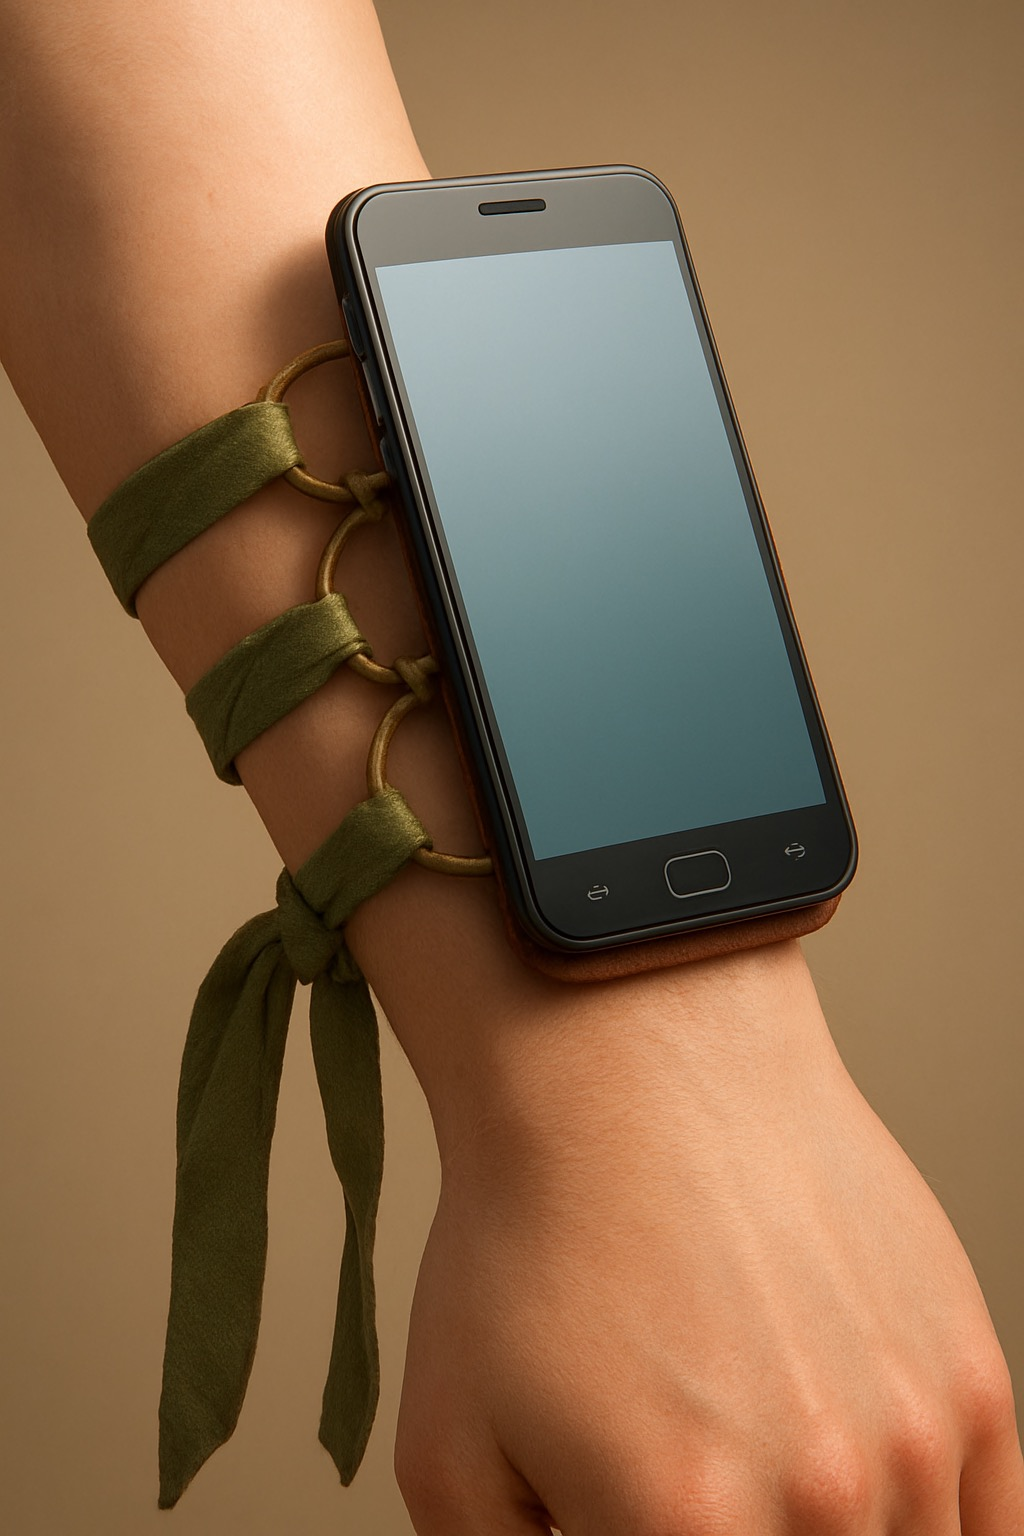
\includegraphics[width=0.65\textwidth]{Brazalete.png}
    \caption{Visualización conceptual del sostén corporal del dispositivo.
    }
\end{figure}
\vspace{\sectionsep}

\newpage
\begin{figure}[h!]
    \centering
    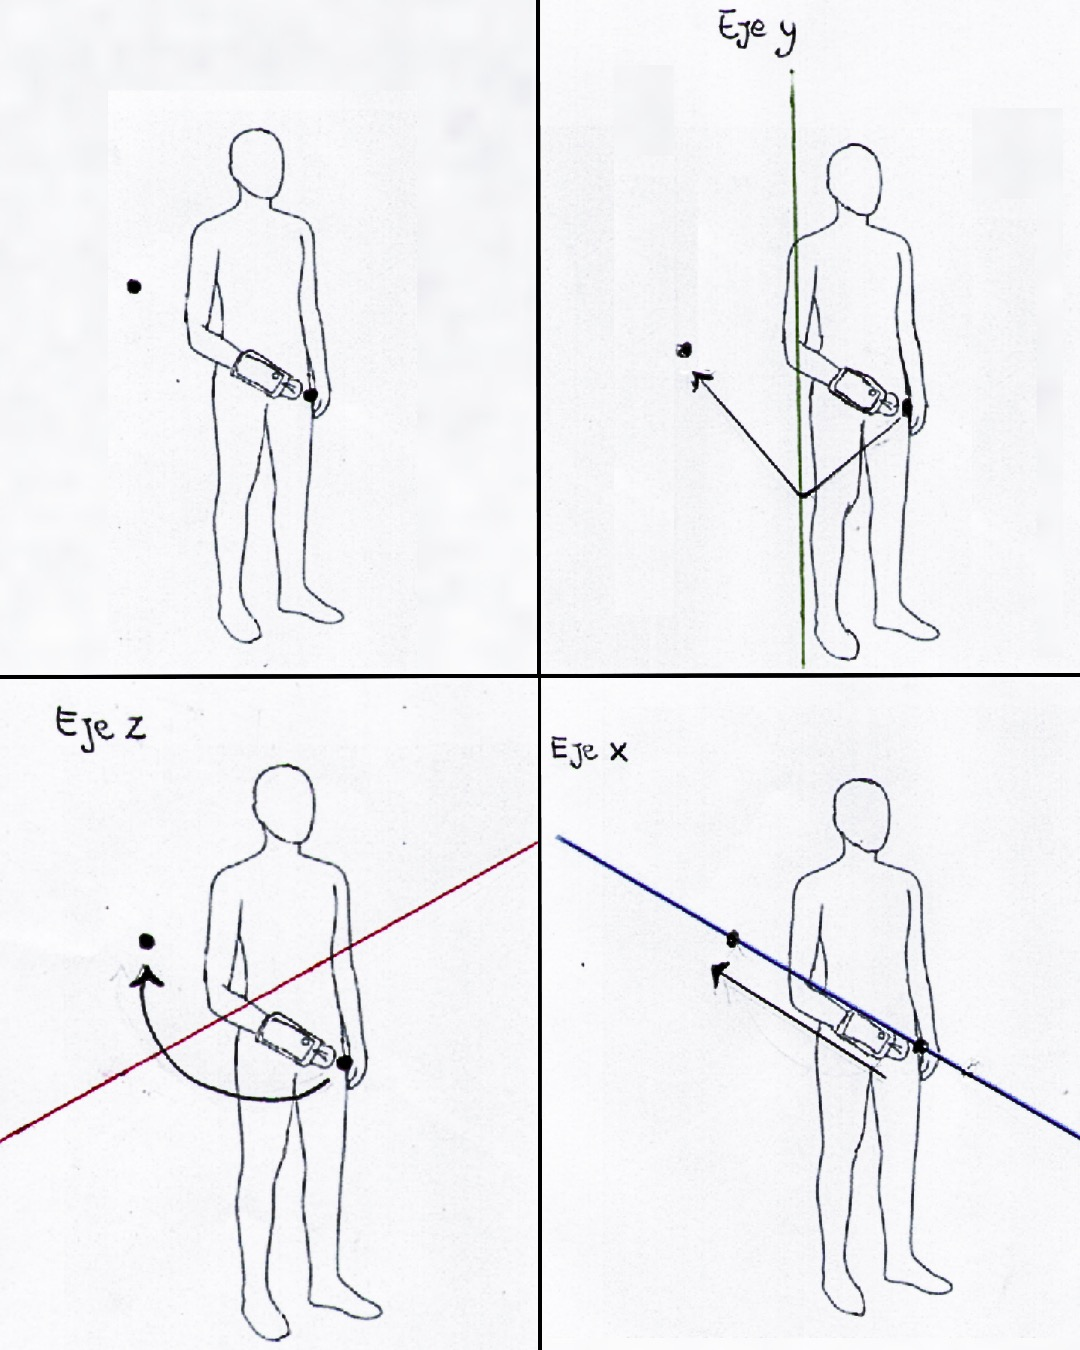
\includegraphics[width=0.65\textwidth]{ejes.png}
    \caption{Representación de los ejes de movimiento entre dos puntos imaginarios en el espacio. x, y, z. 
    }
\end{figure}
\vspace{\sectionsep}

\begin{center}
\begin{tcolorbox}[
            breakable,
            title=Partitura Instructiva de Celuido,
            colback=gray!5,
            colframe=black,
            fonttitle=\bfseries,
            arc=2mm,
            boxrule=0.5pt
        ]

        \section*{Primera parte}

        \subsection*{Preparación}

        Estar de pie o sentade, con el brazo libre.  
        Percibir la respiración.

        \medskip

        \subsection*{Dirección}

        Localizar una línea imaginaria entre el codo y la mano.  
        Esa línea puede orientarse en cualquier eje del espacio: horizontal (X), vertical (Y) o de profundidad (Z).

        Imaginar dos puntos en el espacio.  
        El movimiento entre esos puntos puede ser \textbf{lineal} (horizontal o vertical)  
        o \textbf{curvo} (vertical o profundidad).

        Repetir hasta tres veces, si la atención se sostiene.

        \bigskip

        \section*{Segunda parte}

        \subsection*{Profundidad}

        Imaginar puntos muy cercanos entre sí.  
        Imaginar un punto adelante y otro detrás del cuerpo.  
        Imaginar puntos muy lejanos entre sí.

        \medskip

        \subsection*{Velocidad}

        Explorar distintas velocidades.  
        Moverse entre puntos lo más rápido posible.  
        Moverse entre puntos lo más lento posible.  
        Alternar entre ambas.

        \medskip

        \subsection*{Escucha}

        Escuchar antes de moverse.  
        Escuchar durante el movimiento.  
        Escuchar después.  
        Si no hay nada que escuchar, esperar.

        \bigskip

        \section*{Tercera parte}

        \subsection*{Observación}

        Observar un movimiento antes de moverse.  
        Si no hay nada que observar, iniciar el movimiento.  
        Imitar el movimiento.  
        Acelerar el movimiento.  
        Realizar el movimiento lo más lento posible.

        \medskip
        \subsection*{Cierre}

        Detener el movimiento cuando se disuelva la atención.  
        Volver a la respiración.
\end{tcolorbox}
\captionof{figure}{Partitura Instructiva de Celuido}    
\end{center}

\begin{figure}[h!]
    \centering
    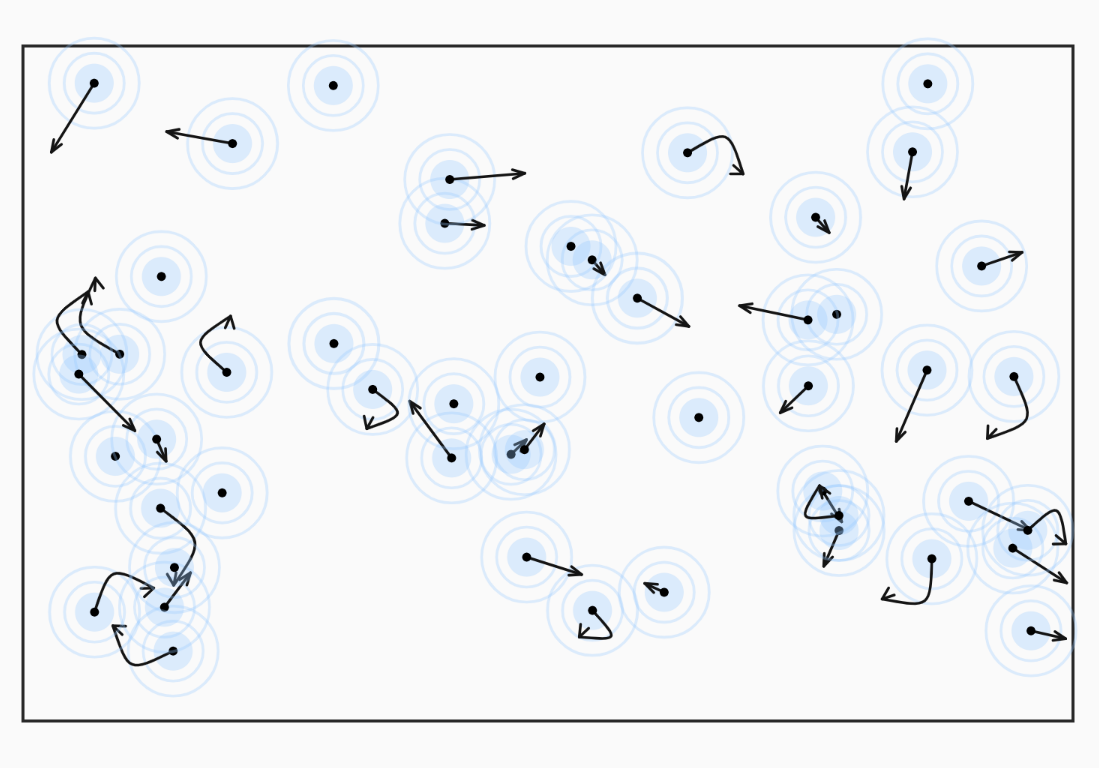
\includegraphics[width=0.65\textwidth]{Movimientos.png}
    \caption{Distribución espacial de participantes y vectores de desplazamiento asociados al uso del celular como dispositivo lumínico y sonoro.
    }
\end{figure}
\vspace{\sectionsep}


% -------------------------
% 6. DESARROLLO
% -------------------------
\newpage
\vspace{\sectionsep}
\section{Desarrollo}
El proyecto está pensado en 4 etapas:
 \begin{itemize}
    \item Investigación.
    Explorar la creación de un instrumento a partir de criterios organológicos, integrando las capacidades tecnológicas del dispositivo y expandiendo su apariencia, su funcionamiento técnico, su técnica interpretativa y su producción sonora y lumínica.
    
    La investigación examina su condición instrumental atendiendo a las diferencias y correspondencias con instrumentos tradicionales y dispositivos electrónicos actuales, con el propósito de expandir la concepción de qué es un celular y qué es un instrumento musical, y de qué modo estas definiciones abren nuevas posibilidades para la práctica musical.

    \item Prototipado.
    Desarrollo del instrumento, del sostén para el dispositivo y de la partitura de la obra, y de las instrucciones para quien vaya a guiar la obra.

    \item Pruebas preliminares y documentación.

    \item Implementación y Divulgación.
 \end{itemize}

\vspace{\sectionsep}

\newpage
\subsection{Cronograma}

\begin{center}
% Ajustá la escala vertical si el Gantt queda muy alto:
% - Cambiá y unit chart (ej. 0.5cm -> 0.45cm o 0.4cm)
% - Cambiá las fuentes de labels a \scriptsize si hace falta
\resizebox{\textwidth}{!}{%
\begin{ganttchart}[
    hgrid,
    vgrid,
    compress calendar,
    time slot format=isodate,
    x unit=0.065cm,
    y unit chart=0.5cm,           % <-- reducilo si es muy alto (ej. 0.45cm)
    milestone label font=\footnotesize,
    bar label font=\footnotesize,
    group label font=\footnotesize\bfseries,
    % opcional: reduce labels automáticamente si hace falta:
    % milestone label node/.append style={font=\scriptsize},
    % bar label node/.append style={font=\scriptsize}
]{2026-02-01}{2026-06-30}
    \gantttitle{Cronograma general del proyecto}{150} \\
    \gantttitlecalendar{year, month=name} \\
    \ganttgroup{Fase 1: Investigación}{2026-02-01}{2026-03-30} \\
    \ganttbar{Relevamiento teórico y referencias}{2026-02-01}{2026-02-20} \\
    \ganttbar{Definición de caso de uso y entorno}{2026-02-15}{2026-02-30} \\
    \ganttgroup{Fase 2: Prototipo técnico}{2026-03-01}{2026-04-15} \\
    \ganttbar{Diseño de interacción y mapeos}{2026-03-01}{2026-04-20} \\
    \ganttbar{Implementación hardware/software}{2026-03-15}{2026-04-20} \\
    \ganttgroup{Fase 3: Pruebas con público}{2026-04-20}{2026-05-30} \\
    \ganttbar{Test interno y ajuste fino}{2026-05-15}{2026-06-05} \\
    \ganttbar{Sesiones piloto con usuarios}{2026-05-20}{2026-06-05} \\
    \ganttgroup{Fase 4: Implementación y divulgación}{2026-06-05}{2026-06-30} \\
    \ganttbar{Instrucción a les guías.}{2026-06-16}{2026-06-19} \\
    \ganttbar{Exhibición y documentación}{2026-06-19}{2026-06-30} \\
    \ganttmilestone{Entrega de informe final}{2026-06-30}
\end{ganttchart}%
} % fin resizebox
\par\medskip
\captionof{figure}{Cronograma general del proyecto.}
\end{center}

\vspace{3em}
\begin{center}
\begin{tabular}{lccccccc}
    \hline
    Rubro / Mes & Feb & Mar & Abr & May & Jun \\
    \hline
    Investigación teórica         & X &  &   &   &   &   &   \\
    Desarrollo de software        &   & X & X &   &   \\
    Prototipado físico            &   &   & X & X &  &   &   \\
    Instruccion a les guías              &   &   &   &   & X    \\
    Difusión y comunicación       &   &   &   &  & X  \\
    \hline
\end{tabular}
\vspace{1em}

\captionof{figure}{Cronograma por rubro y mes. La X indica la actividad principal en cada período.}
\end{center}


% -------------------------
% 7. LISTA DE MATERIALES
% -------------------------
\vspace{\sectionsep}
\section{Lista de materiales}
La obra requiere un conjunto reducido de materiales, centrados exclusivamente en el uso de dispositivos móviles del público. Para su correcta implementación, solo se necesitan sostenes/soportes para celulares: destinados a asegurar la correcta posición, estabilidad y visibilidad del dispositivo durante la activación de la obra.


% -------------------------
% 8. RIDER
% -------------------------
\vspace{\sectionsep}
\section{Rider}

\begin{center}
\begin{figure}[h!]
    \centering
    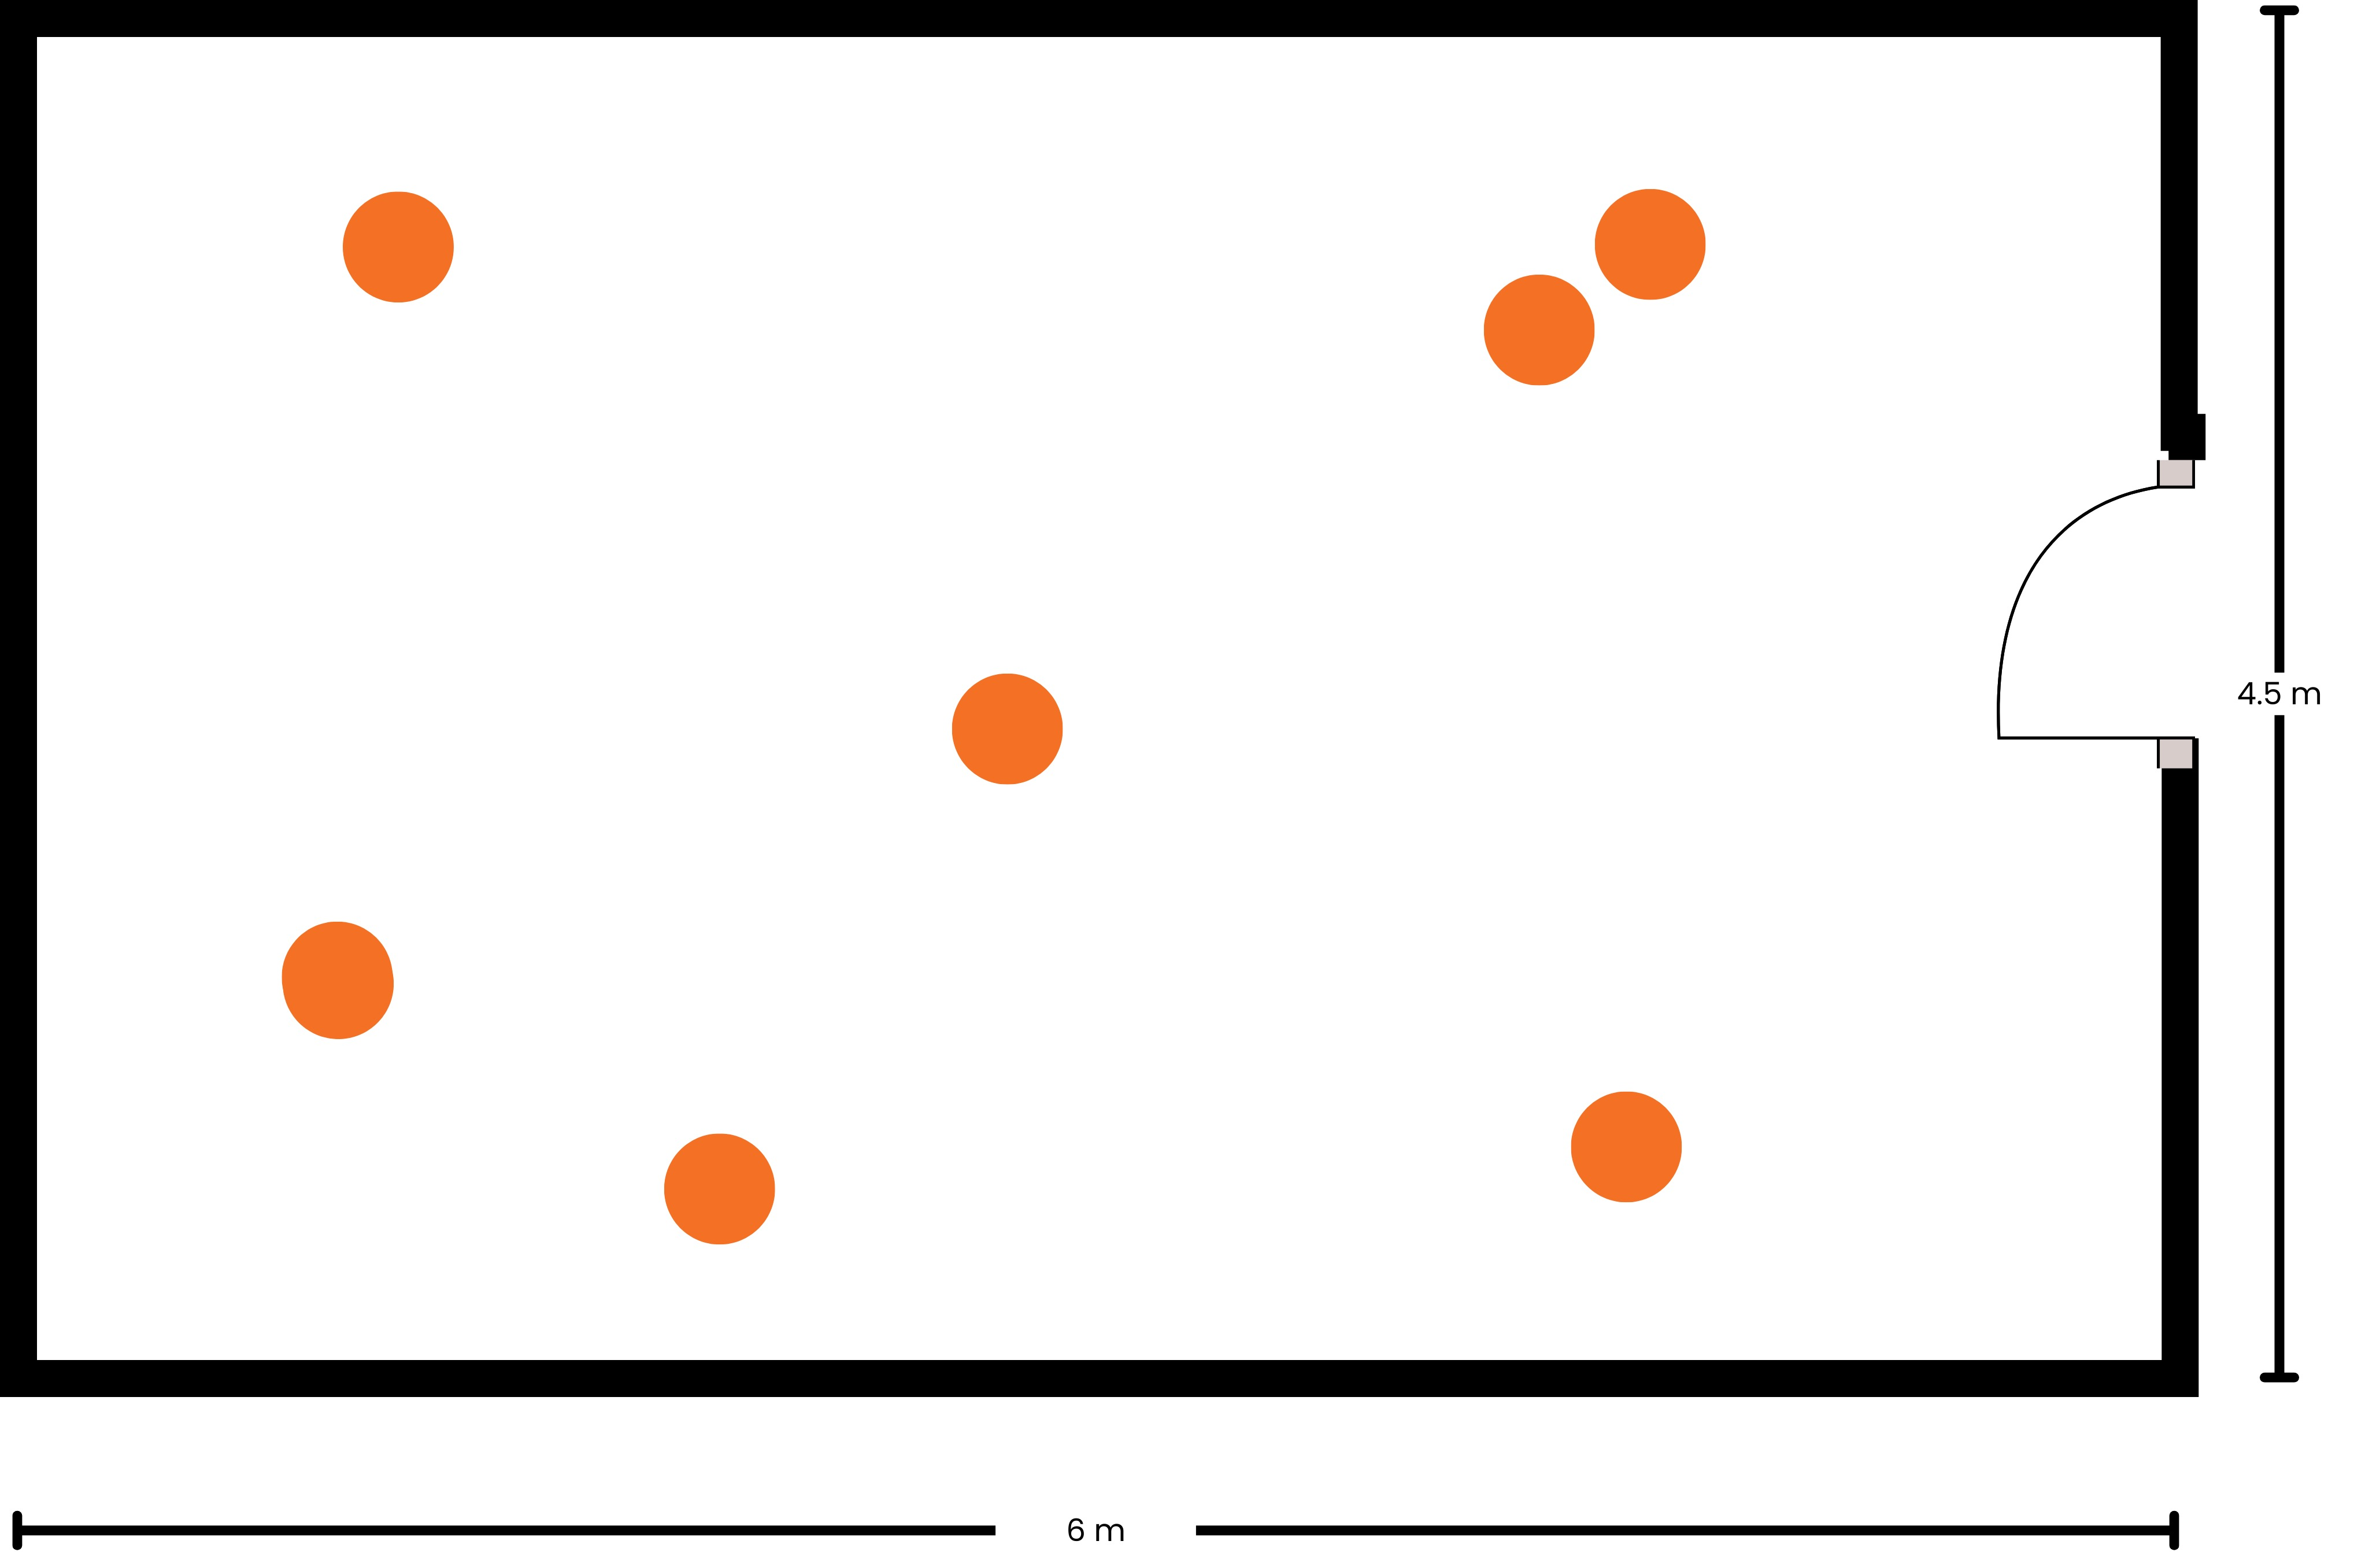
\includegraphics[width=0.65\textwidth]{Plano de la sala.png}
    \caption{Plano de la sala.}
\end{figure}
\end{center}

Se necesita una habitación vacía, silenciosa y alejada de ruidos del entorno. El espacio debe permitir el movimiento cómodo de los cuerpos, por lo que se recomienda una superficie libre no menor a 6 × 4.5 metros, aunque esto va a depender del número de participantes. En caso de que las presentaciones con grupos numerosos sean frecuentes, se recomienda contemplar un espacio proporcionalmente mayor que garantice comodidad y libertad de movimiento.

La iluminación debe ser tenue o baja, evitando luces directas o cambios bruscos de luminosidad. Se sugiere que la sala se mantenga a una temperatura calida y estable, entre 20 y 24°C, para favorecer la permanencia del público y el uso de los dispositivos móviles.

La obra utiliza únicamente los teléfonos celulares del público y sus respectivos soportes, no se requiere equipamiento adicional.


% -------------------------
% 10. PRESUPUESTO
% -------------------------
\vspace{\sectionsep}
\section{Presupuesto}
\begin{table}[h!]
    \centering
    \begin{tabular}{lrrrr}
        \hline
        Rubro & Costo unitario (USD) & Cantidad & Subtotal (USD) \\
        \hline
        Diseño y prototipado físico          & 274  & 1   & 274  \\
        Confección de prototipado físico     & 120  & 25  & 3000 \\
        Honorarios artista                   & 798  & 1   & 798  \\
        Diseño de comunicación               & 98   & 1   & 98   \\
        Gastos en difusión                   & 96   & 1   & 96   \\
        \hline
        Total estimado                      &      &     & 4266 \\
        \hline
    \end{tabular}
    \caption{Presupuesto preliminar por rubro. Los valores son orientativos.} 
\end{table}

El ítem de diseño y prototipado físico corresponde a un trabajo colaborativo realizado con une diseñador, que se va a encargar de desarrollar tanto la concepción como los primeros modelos del instrumento. Por otro lado, el prototipado físico hace referencia a la confección de los sostenes para el dispositivo, que se colocan en el brazo de cada participante. Se estima la producción de una cantidad aproximada de 25 unidades, aunque esta cifra puede ajustarse según la cantidad de público o participantes que se esperen.

Los honorarios contemplados están basados en las tarifas vigentes del TAV, actualizadas para octubre de 2025, y corresponden a la remuneración por la labor artística involucrada en el proyecto. En cuanto al diseño de comunicación, este rubro incluye la creación de materiales gráficos como flyers y contenido para redes sociales, mientras que los gastos en difusión cubren la publicidad y promoción del evento o la obra. Es importante destacar que estos últimos costos podrían ser absorbidos por la institución.

% -------------------------
% 11. REFERENCIAS / COMUNICACIÓN
% -------------------------
\vspace{\sectionsep}
\section{Referencias y comunicación}

\subsection{Bibliografía}
\renewcommand{\refname}{}
\renewcommand{\bibname}{}
\let\oldclearpage\clearpage
\let\clearpage\relax
\vspace{-8em} 
\begin{thebibliography}{1}
\bibitem{forsythe}
Forsythe, William. ``Choreographic Objects.'' Ensayo publicado en línea, William Forsythe Studio. \url{https://www.williamforsythe.com/essay.html}. Consultado 25 nov. 2025.

\bibitem{oliveros}
Oliveros, Pauline. \textit{Deep Listening: A Composer’s Sound Practice}. Bloomington, IN: iUniverse, 2005.

\bibitem{fuller}
Fuller, Matthew, y Usman Haque (2008). \textit{Urban Versioning System (UVS)}. En O. Khan, T. Scholz, \& M. Shepard (Eds.), \textit{Situated Technologies Pamphlets}. The Architectural League of New York.

\bibitem{wagner}
Wagner, Phoebe, y Brontë Christopher Wieland, eds. \textit{Sunvault: Stories of Solarpunk and Eco-Speculation}. Pittsburgh: Upper Rubber Boot Books, 2017.

\bibitem{levin}
Levin, Golan. (2007, 27 de agosto). \textit{Mobile Phone Concert: Dialtones @ Ars Electronica 2001}. YouTube. \url{https://www.youtube.com/watch?v=g1G-YesiBB8}. Consultado 25 nov. 2025.

\end{thebibliography}
\let\clearpage\oldclearpage

\subsection{Teaser}
Celuido una performance de sonificación e iluminación colectiva generada por el movimiento de los brazos a partir del celular como sensor.

Se brindará un sistema de reglas que funciona como disparador para pensar la meditación que deviene en improvisación de movimiento, música y luz.  


\subsection{Statement}
Como estudiante universitaria en una institución pública actualmente bajo ataque, mi cotidianeidad se encuentra atravesada por procesos sostenidos de precarización, agotamiento y desánimo. Habito en José C. Paz, una localidad de la provincia de Buenos Aires donde la pobreza alcanza al 31\% de la población y donde han resurgido prácticas comunitarias como el trueque —intercambio de mercadería, prendas, medicamentos o herramientas— que funcionan como estrategias colectivas de sostenimiento en escenarios de crisis. Estas formas de organización solidaria muestran que, aun en contextos adversos, emergen modos alternativos de habitar lo cotidiano.

En paralelo, mi formación en una carrera cuyo eje fundante es la creación musical me enseñó desde el inicio a partir de lo conocido para expandirlo hacia sus potencialidades no exploradas. Ese enfoque, orientado a transformar lo dado y abrir nuevos sentidos, adquiere especial relevancia en un entorno social que exige formas constantes de reinvención. Es justamente en la intersección entre este contexto social y mi práctica creativa donde surge la idea de concebir un instrumento y una obra.

En este marco aparece la decisión de trabajar con el teléfono celular. Se trata de un dispositivo prácticamente universal, independientemente de la edad, la formación o la situación socioeconómica. Su presencia transversal lo convierte no solo en una herramienta técnica, sino en un soporte cultural compartido, profundamente integrado a la vida cotidiana. Trabajar con el celular como material e interfaz permite así partir de un objeto accesible, conocido y disponible, y activar nuevas posibilidades de creación sin requerir recursos adicionales ni conocimientos especializados.

Sin embargo, incorporar el celular como soporte creativo plantea dos desafíos centrales: por un lado, la necesidad de reconfigurar las acciones y significados con los que el dispositivo está habitualmente asociado; por otro, la tarea de transformarlo en un instrumento musical, lo que implica redefinir sus funciones, modos de interacción y capacidades expresivas.

Más allá de sus potencialidades técnicas, el teléfono celular porta una carga cultural ambivalente: es un objeto íntimo y cotidiano, pero también un símbolo de control, hiperconectividad, dependencia, distracción y productividad forzada. No se trata de negar estas dimensiones, sino de reconocer que configuran el modo en que el dispositivo se inscribe en los cuerpos y en las prácticas sociales. El desafío consiste en correrse de esos significados hegemónicos para abrir un uso alternativo: un imaginario en el cual el celular deje de operar únicamente como terminal de consumo o canal de vigilancia, y se convierta en un espacio de experimentación sensible y de agencia creativa.

En ese desvío también aparece una fuga: no solo en el sentido musical, sino como un escape deliberado del imaginario dominante que rodea al celular dentro del sistema capitalista. Si al comienzo hablaba del trueque como una microfisura capaz de abrir otro régimen de relaciones, aquí el gesto es similar: tomar un objeto cotidiano saturado de usos productivistas, ansiedades y automatismos, y desviarlo hacia otra ética de funcionamiento. Mi obra no busca negar la carga cultural del celular, sino filtrarla, reescribirla, torcerla. Insistir en su uso creativo es afirmar que, incluso dentro de la maquinaria del presente, existen fibras disponibles para tejer otros modos de habitar el tiempo y el espacio. No se trata simplemente de transformar al celular en un instrumento, sino de desplegarlo como un dispositivo abierto: un territorio para la meditación, para la escucha colectiva, para imaginar futuros y tomar conciencia de los cuerpos que co-presencian un mismo espacio.

En ese horizonte, lo solarpunk aparece como una brújula posible: una mirada que invita a pensar tecnologías capaces de reorientarse hacia prácticas cooperativas, lúdicas y sensibles. Mi obra se inscribe allí como un gesto mínimo pero insistente hacia ese futuro posible (y también confío en el efecto mariposa!!!).

\end{document}